% ══════════════════════════════════════════════════════════════════════════════
% CHAPTER 4 — DATA  [fully checked against latest data-check output]
% ══════════════════════════════════════════════════════════════════════════════

This chapter describes the data inputs used in the empirical analysis. It covers the
central bank text corpus (Section~\ref{sec:data_text}), the text preprocessing and
cleaning pipeline (Section~\ref{sec:data_preprocessing}), high-frequency financial
market data (Section~\ref{sec:data_market}), and hand-coded interest rate decisions
(Section~\ref{sec:data_rates}). Section~\ref{sec:data_sample} explains how these
sources are merged into the regression samples and reports sample attrition.
Section~\ref{sec:data_descriptives} presents descriptive statistics.


% ══════════════════════════════════════════════════════════════════════════════
\section{Textual Corpus}
\label{sec:data_text}
% ══════════════════════════════════════════════════════════════════════════════

The textual corpus consists of \textbf{884 central bank communication documents}
from the Federal Open Market Committee (FOMC) and the European Central Bank
(ECB). For each institution, two document types are used: policy statements and
press conference transcripts. \Cref{tab:corpus_overview} summarises the corpus,
and \Cref{fig:sample_coverage} visualises the coverage of each document type over
time.

\subsection{FOMC Statements}
\label{sec:data_fomc_stmt}

FOMC post-meeting communications are collected from February~1994, when the
Committee first began announcing the outcome of selected meetings, through
March~2026. The resulting corpus contains \textbf{242 statement documents}, covering
scheduled meetings and inter-meeting communications. Each statement is assigned a
unique event identifier constructed from the meeting date, for example
\texttt{fomc\_stmt\_20220316}, and is matched to the corresponding event date in the
financial market data.

The statements are sourced from the pre-compiled file
\texttt{fomc\_statements\_econometrics.csv}, which contains the raw text, meeting
date, speaker or Chair identifier, and central bank identifier. Statements are not
subject to speaker-turn cleaning because they are official committee documents and
do not contain journalist questions. They are nevertheless processed through the
common tokenisation, stop-word removal, and stemming pipeline described in
Section~\ref{sec:data_tokenisation}.

\subsection{FOMC Press Conferences}
\label{sec:data_fomc_pc}

FOMC press conference transcripts are available from April~2011 onward, yielding
\textbf{92 documents}. Press conferences were initially held after four meetings per
year, generally those associated with the Summary of Economic Projections, and were
extended to every scheduled FOMC meeting from January~2019. The transcripts are
sourced from \texttt{fomc\_press\_conferences\_econometrics.csv} and contain the
Chair's opening remarks and the subsequent question-and-answer session.

Because these transcripts contain both central bank communication and journalist
questions, they require speaker-turn cleaning before scoring. The final FOMC press
conference text retains only the Chair's own remarks and answers; journalist
questions and non-Chair speaker turns are removed. The cleaning procedure is
specified in Section~\ref{sec:data_fomc_pc_clean}.

\subsection{ECB Statements}
\label{sec:data_ecb_stmt}

ECB statements refer to the introductory monetary policy statement read by the ECB
President at the start of each press conference. These statements are collected for
Governing Council monetary policy meetings from January~1999 through March~2026,
yielding \textbf{284 documents}. The statements are sourced from
\texttt{ecb\_decisions\_econometrics.csv} and are mapped in the data pipeline to the
\texttt{ecb\_statements} source label with event identifiers of the form
\texttt{ecb\_stmt\_YYYYMMDD}.

The ECB held monetary policy meetings monthly until the beginning of 2015, producing
a denser early sample than the FOMC, which holds eight scheduled meetings per year.
After the ECB switched to a six-weekly monetary policy meeting schedule in
January~2015, the observation frequency became closer to that of the FOMC.

\subsection{ECB Press Conferences}
\label{sec:data_ecb_pc}

ECB press conference transcripts cover the question-and-answer part of the press
conference following the introductory statement. The raw ECB web pages often contain
both the introductory statement and the Q\&A in a single file. For the empirical
analysis, these objects are separated conceptually: the introductory statement enters
the ECB statement corpus and is matched to the EA-MPD press release window, while
the press conference corpus is intended to capture the official ECB answers during the
Q\&A and is matched to the EA-MPD press conference window.

The ECB press conference corpus contains \textbf{266 documents} from January~1999
through December~2025. This is fewer than the 284 ECB statement documents,
reflecting meetings for which the introductory statement is available but the Q\&A
transcript is missing, not yet covered by the raw corpus, or could not be recovered in
a usable format. The transcripts are sourced from
\texttt{ecb\_statements\_econometrics.csv} and mapped to the
\texttt{ecb\_press\_conferences} source label with event identifiers of the form
\texttt{ecb\_pressconf\_YYYYMMDD}.

A data quality issue affects part of the ECB press conference sample, especially from
2019 onward: some downloaded texts lack explicit \texttt{Question:} labels, which are
needed to distinguish journalist questions from official answers. For affected
transcripts, the pipeline re-scrapes the formatted HTML from \texttt{ecb.europa.eu},
uses the HTML structure to recover speaker labels, and caches the downloaded pages
locally in \texttt{ecb\_html\_cache.rds}. The cache contains \textbf{54 successfully
fetched transcripts}, all of which are reused by the current data pipeline. This
procedure reduces repeated web requests and makes the cleaning step reproducible
once the cache has been created.

In addition to the HTML re-scraping described above, a targeted
recovery step attempts to fetch the raw text of documents that
remained missing or truncated (fewer than 100 characters) after the
initial corpus assembly. The recovery targets two FOMC statements
(\texttt{fomc\_stmt\_20070628} and \texttt{fomc\_stmt\_20080122})
and eight ECB statements from 1999--2006 for which the pre-compiled
CSV contained no usable text. Of these ten targets, the two FOMC
statements and a subset of the ECB statements were successfully
recovered from the central bank websites. The recovered texts are
merged back into the corpus; documents that could not be recovered
are retained with missing text and are excluded from subsequent
scoring and regression analyses.

\subsection{Corpus Overview}

\begin{table}[htbp]
\centering
\caption{Textual corpus overview}
\label{tab:corpus_overview}
\begin{threeparttable}
\small
\begin{tabular}{llcrr}
\toprule
Central bank & Document type & Period & $N$ & Avg. tokens\tnote{a} \\
\midrule
FOMC & Statement        & 1994--2026 & \textbf{242} & 223 \\
FOMC & Press conference & 2011--2026 & \textbf{92}  & 2{,}325 \\
ECB  & Statement        & 1999--2026 & \textbf{284} & 109 \\
ECB  & Press conference & 1999--2025 & \textbf{266} & 1{,}776 \\
\midrule
     & \textbf{Total}   &            & \textbf{884} & \\
\bottomrule
\end{tabular}
\begin{tablenotes}\footnotesize
  \item[a] Average non-stopword token count after cleaning and preprocessing. For
  press conferences, journalist questions are excluded from the cleaned text.
\end{tablenotes}
\end{threeparttable}
\end{table}

% --------------------------------------------------------------------------
% Figure 4.1 — compact coverage timeline
% Data checked against fig_4_1_sample_coverage_intervals.csv:
% FOMC statements:        1994-02-04 to 2026-03-18, N = 242
% FOMC press conferences: 2011-04-27 to 2026-03-18, N = 92
% ECB statements:         1999-01-07 to 2026-03-19, N = 284
% ECB press conferences:  1999-01-07 to 2025-12-18, N = 266
% --------------------------------------------------------------------------
\begin{figure}[htbp]
\centering
\resizebox{0.96\textwidth}{!}{%
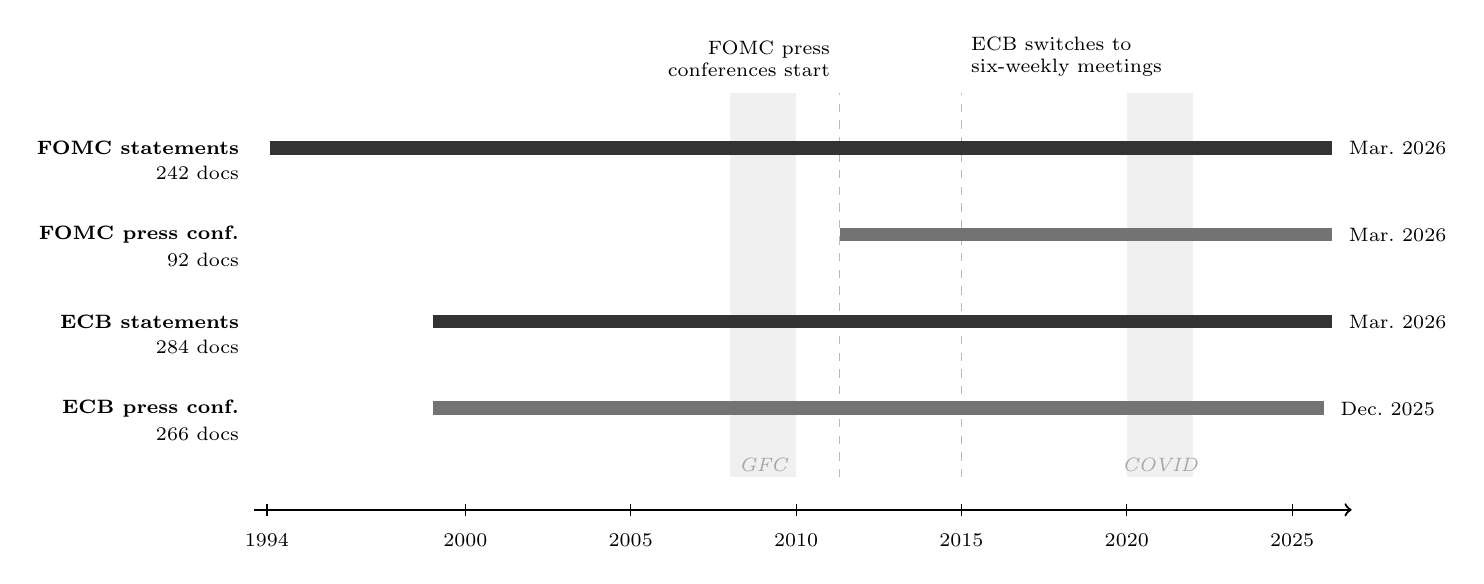
\begin{tikzpicture}[
  xscale=0.42,
  yscale=0.92,
  every node/.style={font=\scriptsize}
]
  % Coordinate system: x = calendar year - 1994.
  \draw[->, thick] (-0.4,-0.8) -- (32.8,-0.8);
  \foreach \year in {1994,2000,2005,2010,2015,2020,2025} {
    \pgfmathsetmacro{\xpos}{\year-1994}
    \draw (\xpos,-0.88) -- (\xpos,-0.72);
    \node[below=3pt] at (\xpos,-0.88) {\year};
  }

  % Crisis shading.
  \fill[gray!12] (14.0,-0.35) rectangle (16.0,4.95);
  \fill[gray!12] (26.0,-0.35) rectangle (28.0,4.95);
  \node[gray!70, font=\scriptsize\itshape] at (15.0,-0.18) {GFC};
  \node[gray!70, font=\scriptsize\itshape] at (27.0,-0.18) {COVID};

  % Structural break lines.
  \draw[gray!55, thin, dashed] (17.32,-0.35) -- (17.32,4.95);
  \draw[gray!55, thin, dashed] (21.00,-0.35) -- (21.00,4.95);
  \node[anchor=south east, align=right] at (17.32,5.05) {FOMC press\\conferences start};
  \node[anchor=south west, align=left] at (21.00,5.05) {ECB switches to\\six-weekly meetings};

  % Coverage bars.
  \draw[line width=5pt, black!80] (0.09,4.20) -- (32.21,4.20);
  \draw[line width=5pt, black!55] (17.32,3.00) -- (32.21,3.00);
  \draw[line width=5pt, black!80] (5.02,1.80) -- (32.21,1.80);
  \draw[line width=5pt, black!55] (5.02,0.60) -- (31.96,0.60);

  % Labels.
  \node[anchor=east, font=\scriptsize\bfseries] at (-0.55,4.20) {FOMC statements};
  \node[anchor=east] at (-0.55,3.85) {242 docs};
  \node[anchor=east, font=\scriptsize\bfseries] at (-0.55,3.00) {FOMC press conf.};
  \node[anchor=east] at (-0.55,2.65) {92 docs};
  \node[anchor=east, font=\scriptsize\bfseries] at (-0.55,1.80) {ECB statements};
  \node[anchor=east] at (-0.55,1.45) {284 docs};
  \node[anchor=east, font=\scriptsize\bfseries] at (-0.55,0.60) {ECB press conf.};
  \node[anchor=east] at (-0.55,0.25) {266 docs};

  % Endpoint labels.
  \node[anchor=west] at (32.42,4.20) {Mar.~2026};
  \node[anchor=west] at (32.42,3.00) {Mar.~2026};
  \node[anchor=west] at (32.42,1.80) {Mar.~2026};
  \node[anchor=west] at (32.17,0.60) {Dec.~2025};
\end{tikzpicture}%
}
\caption[Sample coverage timeline]{Sample coverage timeline, 1994--2026. Bars show
the available text coverage for each corpus. Grey bands indicate the Global Financial
Crisis and the COVID-19 period. Dashed lines mark the start of the FOMC press
conference sample in April~2011 and the ECB's switch to six-weekly monetary policy
meetings in January~2015. Exact document counts are reported in
\Cref{tab:corpus_overview}.}
\label{fig:sample_coverage}
\end{figure}


% ══════════════════════════════════════════════════════════════════════════════
\section{Text Preprocessing}
\label{sec:data_preprocessing}
% ══════════════════════════════════════════════════════════════════════════════

The preprocessing pipeline has two purposes. First, it removes text that does not
represent central bank communication, especially journalist questions and
institutional boilerplate. Second, it converts the remaining text into a form suitable
for dictionary scoring and machine-learning feature extraction. Statements require no
speaker-turn cleaning, while press conference transcripts require more extensive
processing because they contain multiple speakers.

\subsection{ECB Press Conference Cleaning}
\label{sec:data_ecb_pc_clean}

ECB press conference transcripts contain official ECB communication and journalist
questions. Since journalist questions do not represent the ECB's policy stance, they are
removed before scoring. The cleaned press conference text is designed to retain official
answers by the President, Vice-President, Chief Economist, or other identifiable ECB
officials, while excluding journalist questions and boilerplate.

The cleaning algorithm proceeds in four steps. First, institutional boilerplate is
removed from the end of each transcript, including footer material containing phrases
such as ``CONTACT European Central Bank,'' ``Disclaimer,'' and ``Reproduction is
permitted.'' Second, the algorithm identifies the start of the Q\&A section. Text before
the first question label is not treated as press-conference Q\&A text. Third, labelled
speaker turns are detected using a regular expression that matches question labels and
the surnames of known ECB officials, including Duisenberg, Trichet, Draghi, Lagarde,
Noyer, Papademos, Constâncio, de~Guindos, and Lane. Fourth, question segments are
discarded and official response segments are concatenated into the final cleaned press
conference text. Where the raw downloaded text lacks reliable question labels, the
pipeline uses the locally cached HTML recovery procedure described in
Section~\ref{sec:data_ecb_pc}.

\Cref{tab:ecb_pc_cleaning} reports cleaning diagnostics from the current data run. The
most important diagnostic is not the mean retention rate alone, but the combination of
retention, high-retention flags, and over-cleaning flags. High-retention observations are
not automatically errors: some press conferences contain long official answers relative to
journalist questions. However, documents retaining more than 95\% of the raw text are
flagged for inspection because they may indicate that question labels were not detected.

\begin{table}[htbp]
\centering
\caption{ECB press conference cleaning diagnostics}
\label{tab:ecb_pc_cleaning}
\begin{tabular}{lr}
\toprule
Metric & Value \\
\midrule
Transcripts cleaned                         & 266 \\
Mean text retained                          & 82.0\% \\
Median text retained                        & 78.9\% \\
Documents $>$95\% retained                  & 65 \\
Documents $<$20\% retained                  & 0 \\
HTML transcripts recovered and cached       & 54 \\
\bottomrule
\end{tabular}
\end{table}

The realised mean retention rate of 82.0\% is above the initial target range of
40--70\%. This should not be interpreted as automatic validation of the cleaning
procedure. Instead, it indicates that the ECB corpus contains a non-trivial set of
high-retention documents, mostly around the period where the downloaded texts no
longer contain explicit \texttt{Question:} labels. These cases are handled by the HTML
re-scraping procedure described in Section~\ref{sec:data_ecb_pc}. The absence of any
document below the 20\% threshold indicates that the algorithm does not aggressively
over-cut the corpus, but the high-retention cases remain the more relevant diagnostic
risk.

\subsection{FOMC Press Conference Cleaning}
\label{sec:data_fomc_pc_clean}

FOMC press conference transcripts use a different labelling convention. Speakers are
identified by capitalised labels, such as ``CHAIR POWELL.'', and journalist questions are
marked by labels such as ``QUESTION.'' The cleaning algorithm identifies speaker turns
using a regular expression that matches either \texttt{QUESTION.} or a sequence of
capitalised words followed by a period. Only segments attributed to the Chair are
retained; journalist questions and any other speaker turns are discarded.

Across the \textbf{92 FOMC press conferences} in the text corpus, \textbf{91} are matched
to the press-conference market-data window. The cleaned FOMC press conference corpus
has an average post-cleaning length of \textbf{2{,}325 non-stopword tokens}; the
document-length sample reported in \Cref{tab:text_desc} contains \textbf{91} observations
because one document does not survive the final text-score construction filters used in
the descriptive-statistics table. The FOMC cleaning behaves more consistently than the
ECB cleaning because FOMC transcripts use more stable speaker labels.

\subsection{Cleaning Validation}
\label{sec:data_cleaning_validation}

Cleaning can affect measured tone if journalist questions contain systematic hawkish or
dovish language. The pipeline therefore validates press conference cleaning by comparing
dictionary scores computed on raw and cleaned texts. The validation uses the final
dictionary score from the current model,
\[
  \texttt{net\_score} = \frac{H-D}{H+D+10},
\]
where \(H\) and \(D\) are the total hawkish and dovish bigram/trigram matches,
respectively. Labels are assigned using the final threshold of \(\pm 0.05\):
scores above \(0.05\) are labelled hawkish, scores below \(-0.05\) are labelled dovish,
and scores in between are labelled neutral.

Three diagnostics are reported. First, the raw-clean score correlation measures whether
cleaning preserves the relative ranking of documents. Second, the mean score shift
measures whether cleaning moves scores systematically in a hawkish or dovish direction.
Third, the label-flip rate counts the share of documents whose hawkish/neutral/dovish
label changes after cleaning.

\begin{table}[htbp]
\centering
\caption{Effect of text cleaning on dictionary scores}
\label{tab:cleaning_validation}
\begin{threeparttable}
\small
\begin{tabular}{lrrrrrr}
\toprule
Corpus & $N$ & Mean raw & Mean clean & Shift & Corr. & Flips (\%) \\
\midrule
FOMC press conference & 92  & 0.0536 & 0.0573 & 0.0037 & 0.962 & 20.7 \\
ECB press conference  & 266 & 0.0022 & 0.0215 & 0.0193 & 0.980 & 7.1 \\
\bottomrule
\end{tabular}
\begin{tablenotes}\footnotesize
  \item[] Shift is mean(clean score $-$ raw score). Corr. is the Pearson correlation
  between raw and cleaned \texttt{net\_score}. Flips is the percentage of documents
  whose hawkish/neutral/dovish label changes after cleaning using the final
  \(\pm 0.05\) classification threshold.
\end{tablenotes}
\end{threeparttable}
\end{table}

The cleaning validation indicates that cleaning preserves the cross-document ranking of
tone: raw-clean correlations are 0.962 for FOMC press conferences and 0.980 for ECB
press conferences. Mean score shifts are small in absolute terms, though positive in both
corpora, meaning that removing journalist questions slightly increases measured
hawkishness on average. Label flips are more frequent for FOMC press conferences
(20.7\%) than for ECB press conferences (7.1\%), which means that cleaning is not merely
cosmetic: it can change the discrete classification of some press-conference documents.
For this reason, all main empirical results use the cleaned text, because it is the version
intended to measure central bank communication rather than the full transcript including
journalist questions.

\subsection{Tokenisation and Stemming}
\label{sec:data_tokenisation}
 
After cleaning, all texts pass through a common preprocessing
pipeline. Text is lowercased and tokenised into unigrams, bigrams,
and trigrams using the \texttt{tidytext} package in R. The
remaining tokens are Porter-stemmed using the \texttt{SnowballC}
package \citep{porter1980}. For example, ``raising'', ``raised'',
and ``raises'' are all mapped to the stem ``rais''.
 
The same stemming convention is applied to document tokens and
dictionary terms, but the two scoring pipelines use different
stop-word lists. The \textbf{dictionary scorer} uses a custom
conservative stop list of 44 words, restricted to non-directional
function words (articles, copula verbs, pronouns, and safe
prepositions). Directional words such as ``above,'' ``below,''
``further,'' ``not,'' and ``more'' are deliberately retained
because they form essential components of stance-bearing bigrams
(e.g., ``above target,'' ``further tightening''). The dictionary
phrases themselves are written with these stop words already
stripped, so text and dictionary align after identical stop-word
removal. The \textbf{Random Forest TF-IDF pipeline} uses the
default \texttt{tidytext} stop-word list (174 words), with bigrams
filtered if \emph{either} component is a stop word. This broader
removal is appropriate for the RF because the Lasso pre-selection
and feature-importance ranking provide data-driven protection
against uninformative bigrams.
 
In the final dictionary score, only deduplicated bigram and trigram
dictionary matches are used. The current dictionary (v34) contains
288 raw phrase entries and 282 deduplicated bigram/trigram terms
after preprocessing. For the Random Forest, both components of
each bigram are stemmed before the TF-IDF matrix is constructed.


% ══════════════════════════════════════════════════════════════════════════════
\section{Financial Market Data}
\label{sec:data_market}
% ══════════════════════════════════════════════════════════════════════════════

The market reaction analysis uses asset price changes measured in narrow event windows
around monetary policy announcements. Narrow windows reduce the probability that the
measured price movement reflects unrelated macroeconomic or financial news. Two
purpose-built event-study databases are used: the U.S. Monetary Policy Event-Study
Database for the FOMC and the Euro Area Monetary Policy Database for the ECB.

\subsection{US Monetary Policy Database (USMPD)}
\label{sec:data_usmpd}

Intraday financial market reactions to FOMC announcements are obtained from the U.S.
Monetary Policy Event-Study Database of \citet{acosta2025}.\footnote{The USMPD is
accessed through \texttt{USMPD.xlsx}, with separate sheets for statement and press
conference event windows.} The database provides separate observations for the statement
release and the press conference, allowing the two FOMC communication channels to be
matched to separate event windows.

The following variables are extracted:
 
\begin{description}[noitemsep, leftmargin=2.7cm, font=\normalfont\bfseries]
  \item[MP1] The target-rate surprise, based on the current-month
    federal funds futures contract and scaled to reflect the implied
    surprise in the current policy decision \citep{kuttner2001}. MP1
    is the main control variable in FOMC regressions and is reported
    in basis points.
  \item[S\&P~500] The event-window return on the S\&P~500 equity
    index, measured in percent.
  \item[EUR/USD] The event-window change in the EUR/USD exchange
    rate, measured in percent. An increase denotes euro appreciation
    and dollar depreciation.
  \item[DXY] The event-window change in the U.S. Dollar Index, used
    as a robustness measure for dollar movements. The expected sign
    is opposite to EUR/USD: FOMC hawkishness should increase DXY.
  \item[UST~2Y, 5Y, 10Y, 30Y] Event-window changes in U.S.
    Treasury yields at the 2-year, 5-year, 10-year, and 30-year
    maturities, reported in basis points.
  \item[TIPS~5Y, TIPS~10Y] Event-window changes in 5-year and
    10-year Treasury Inflation-Protected Securities (TIPS)
    breakeven inflation rates, reported in basis points. TIPS
    breakevens measure market-implied inflation compensation and
    provide a channel test: under the standard monetary channel,
    hawkish tone should reduce breakevens, while under the
    information effect of \citet{nakamura2018}, hawkish tone
    signalling economic strength could raise them.
\end{description}

The USMPD also contains statement-window indicators for whether a meeting was
associated with a Summary of Economic Projections (SEP) and whether it was an
unscheduled inter-meeting action. These indicators are retained in the merged data but
are not included in the main regression specifications.

\paragraph{Merging procedure.}
The USMPD is merged with the FOMC text data by meeting date. Each FOMC statement
is matched to the statement-window sheet, and each FOMC press conference is matched
to the press-conference-window sheet. All \textbf{242 FOMC statements} are matched to
the statement-window data. Of the \textbf{92 FOMC press conferences}, \textbf{91} are
matched to the press conference window; the unmatched observation is the most recent
meeting in the text corpus and post-dates the current USMPD release used in the
pipeline.

\subsection{Euro Area Monetary Policy Database (EA-MPD)}
\label{sec:data_eampd}

Market reactions to ECB announcements are obtained from the Euro Area Monetary
Policy Database of \citet{altavilla2019}.\footnote{The EA-MPD is accessed through
\texttt{EA-MPD.xlsx}, using the press release and press conference window sheets.}
A key feature of the EA-MPD is that it separates the ECB announcement day into two
windows: the \textbf{press release window}, covering the publication of the policy
decision, and the \textbf{press conference window}, covering the President's press
conference later on the same day. This separation is central to the empirical design
because it allows the ECB statement and Q\&A channels to be analysed separately.

The following variables are extracted:
 
\begin{description}[noitemsep, leftmargin=2.7cm, font=\normalfont\bfseries]
  \item[OIS\_MP1] The short-maturity OIS surprise used as the ECB
    analogue to MP1. The exact source column is detected by the
    pipeline because EA-MPD column names vary across releases. The
    variable is interpreted as the unexpected component of the
    current policy decision and is measured in basis points.
  \item[SX5E] The event-window return on the Euro~Stoxx~50 index,
    measured in percent.
  \item[SX7E] The event-window return on the Euro~Stoxx Banks index,
    capturing the banking channel of monetary policy transmission in
    the euro area. Euro area banks are particularly sensitive to ECB
    rate decisions due to the direct effect on net interest margins.
  \item[EUR/USD] The event-window change in EUR/USD, measured in
    percent. The sign convention is the same as for the FOMC
    regressions: an increase denotes euro appreciation. The expected
    sign differs by central bank: FOMC hawkishness should reduce
    EUR/USD through dollar appreciation, while ECB hawkishness should
    increase EUR/USD through euro appreciation.
  \item[OIS~2Y, 5Y, 10Y] Event-window changes in euro area OIS
    rates at the 2-year, 5-year, and 10-year maturities, measured
    in basis points.
  \item[DE~2Y, DE~10Y] Event-window changes in German Bund yields
    at the 2-year and 10-year maturities, measured in basis points.
    German Bunds serve as the risk-free benchmark for the euro area.
  \item[IT10Y\_spread] The event-window change in the Italian BTP
    10-year yield minus the German Bund 10-year yield, measured in
    basis points. This sovereign spread captures the financial
    fragmentation channel that is specific to ECB communication,
    particularly during the sovereign debt crisis period. An increase
    denotes widening of the Italian premium relative to Germany.
\end{description}
 
In addition to the press release and press conference window sheets,
the pipeline also extracts data from the EA-MPD's \textbf{Monetary
Event Window} sheet, which captures the combined statement-plus-press-conference
surprise. Variables from this sheet are prefixed with
\texttt{eampd\_event\_} and are available for robustness analysis.
 
\paragraph{Column name detection.}
EA-MPD column names vary across data vintages, for example
\texttt{STOXX50} versus \texttt{SX5E} or alternative OIS maturity
labels. The pipeline therefore uses regular expression matching to
select the appropriate column for each conceptual variable. In the
current data run, the Euro~Stoxx~50 variable is detected as
\texttt{STOXX50}.
 
\paragraph{Date conversion.}
EA-MPD dates are converted to R \texttt{Date} objects before
merging. The pipeline handles both Excel serial dates and
character-formatted dates, including European day-month-year
strings.
 
\paragraph{Merging procedure.}
ECB statements are matched to the press release window, and ECB
press conferences are matched to the press conference window. The
merge is performed on meeting date. Of the \textbf{284 ECB
statements}, \textbf{253} match the press-release market-data
window and enter the controlled press-release sample with a
non-missing OIS\_MP1 surprise. Of the \textbf{266 ECB press
conferences}, \textbf{244} match the press-conference market-data
window and \textbf{243} enter the controlled press-conference
sample with a non-missing OIS\_MP1 surprise. Long-maturity OIS
coverage is more limited: \textbf{113 ECB statements} and
\textbf{105 ECB press conferences} have non-missing OIS~10Y
observations. German Bund and sovereign spread coverage follows a
similar pattern. This smaller long-yield sample is reported
explicitly in \Cref{tab:sample_attrition} and is treated as a
limitation when interpreting ECB yield regressions in
Chapter~\ref{ch:results}.

\subsection{Variable Summary}
\label{sec:data_variable_summary}

\Cref{tab:variable_map} maps the main outcome and control variables across the FOMC
and ECB regressions.

\begin{table}[htbp]
\centering
\caption{Variable mapping across FOMC and ECB regressions}
\label{tab:variable_map}
\small
\begin{tabularx}{\textwidth}{@{} l l X X @{} }
\toprule
Role & Regression label & FOMC & ECB \\
\midrule
Rate surprise control & MP1 / OIS\_MP1
  & Federal funds futures surprise
  & Short-maturity OIS surprise \\
Equity index & S\&P~500 / SX5E
  & S\&P~500 return
  & Euro~Stoxx~50 return \\
Exchange rate & EUR/USD
  & EUR/USD return
  & EUR/USD return \\
Short yield & UST~2Y / OIS~2Y
  & U.S. Treasury 2Y yield change
  & Euro area OIS 2Y change \\
Medium yield & UST~5Y / OIS~5Y
  & U.S. Treasury 5Y yield change
  & Euro area OIS 5Y change \\
Long yield & UST~10Y / OIS~10Y
  & U.S. Treasury 10Y yield change
  & Euro area OIS 10Y change \\
Very long yield & UST~30Y / ---
  & U.S. Treasury 30Y yield change
  & Not available \\
\bottomrule
\end{tabularx}
\end{table}


% ══════════════════════════════════════════════════════════════════════════════
\section{Interest Rate Decisions}
\label{sec:data_rates}
% ══════════════════════════════════════════════════════════════════════════════

Interest rate decisions are hand-coded for FOMC meetings from February~1994 to
March~2026 and ECB Governing Council monetary policy meetings from January~1999 to
March~2026. Each decision is recorded as the change in the relevant policy rate in basis
points, denoted \bpschange{}. A positive value indicates a rate hike, zero indicates a
hold, and a negative value indicates a rate cut.

The decision variable is used in three ways. First, it provides the benchmark for the
agreement analysis in Section~\ref{sec:res_agreement}: a hawkish text label agrees with
the rate decision if the meeting produced a hike, a dovish label agrees if the meeting
produced a cut, and a neutral label agrees if the rate was unchanged. Second, the sign of
\bpschange{} defines the three-class target variable for the Random Forest classifier in
Section~\ref{sec:meth_rf}. Third, the next meeting's rate decision is the dependent
variable in the RQ2 predictive analysis in Section~\ref{sec:meth_rq2}.

\subsection{Rate Decision Distribution}
\label{sec:data_rate_distribution}

\begin{table}[htbp]
\centering
\caption{Rate decision distribution by central bank}
\label{tab:rate_distribution}
\begin{threeparttable}
\begin{tabular}{lrrrrrr}
\toprule
Central bank & Cut & Hold & Hike & Total & Hold (\%) & Median $|\Delta|$\tnote{a} \\
\midrule
FOMC & 40 & 147 & 51 & 238 & 61.8\% & 25 bps \\
ECB  & 35 & 221 & 28 & 284 & 77.8\% & 25 bps \\
\bottomrule
\end{tabular}
\begin{tablenotes}\footnotesize
  \item[a] Median absolute size of non-zero rate changes. The FOMC total is below
  the 242-text-document count because four FOMC statement documents are retained in
  the text corpus but do not enter the hand-coded rate-decision calendar used for
  agreement, Random Forest training, and RQ2.
\end{tablenotes}
\end{threeparttable}
\end{table}

The distribution is highly imbalanced. Holds account for 61.8\% of FOMC meetings and
77.8\% of ECB meetings. This imbalance is central for the Random Forest design: a
standard classifier could obtain superficially high overall accuracy by predicting the
majority hold class, while performing poorly on the cut and hike classes that are most
important for hawkish--dovish classification.

Two features of the rate-decision data are relevant for interpretation. First, FOMC rate
changes are recorded in 25-basis-point increments, with the largest cuts in the sample
being 100 basis points in December~2008 and March~2020. Second, the ECB data include
non-standard rate changes of 5 and 10 basis points during the negative-rate period,
reflecting adjustments to the deposit facility rate. For classification, all negative changes
are grouped into the cut class and all positive changes into the hike class, regardless of
magnitude.

\subsection{Propagation to Press Conferences}
\label{sec:data_rate_propagation}

Rate decisions are initially coded at the meeting level and attached to the statement,
because the decision is announced at the statement or press-release stage. To enable
agreement analysis and Random Forest training for press conference documents,
\bpschange{} is propagated from the same-day statement to the corresponding press
conference by a date-based merge. This gives each press conference the rate decision
associated with the meeting at which the press conference took place. Propagated values
are checked against all shared statement--press conference dates.

\subsection{Next-Meeting Rate Decision (RQ2)}
\label{sec:data_rate_rq2}

For RQ2, a chronological meeting calendar is constructed for each central bank. The next
meeting's rate decision, \(\text{bps\_next}_i\), is created using a lead operation, and the
previous meeting's decision, \(\text{bps\_lag1}_i\), using a lag operation. These variables
allow the predictive regressions to test whether forward-looking text predicts the next
rate decision beyond current and lagged policy momentum. The FOMC rate-decision
calendar contains \textbf{238 meetings}; the ECB calendar contains \textbf{284 meetings}.


% ══════════════════════════════════════════════════════════════════════════════
\section{Sample Construction and Attrition}
\label{sec:data_sample}
% ══════════════════════════════════════════════════════════════════════════════

The final regression samples are constructed by merging scored text documents with the
corresponding market data and rate-decision variables, then filtering for non-missing
values of the variables required in each specification. Attrition arises from three sources:
missing text scores, missing event-window market variables, and missing rate-surprise
controls.

For each corpus, two headline market-reaction samples are constructed:

\begin{description}[noitemsep]
  \item[Naive sample:] Requires non-missing \texttt{net\_score}, equity return, and
  EUR/USD return. This sample is used for regressions without the rate-surprise control.
  \item[Controlled sample:] Additionally requires a non-missing MP1 or OIS\_MP1
  rate-surprise control. This is the main RQ1 regression sample.
\end{description}

A separate yield sample is constructed for 10-year yield regressions because long-maturity
coverage differs across databases and starts later for the ECB.

\begin{table}[htbp]
\centering
\caption{Sample construction and attrition}
\label{tab:sample_attrition}
\begin{threeparttable}
\begin{tabular}{lrrrr}
\toprule
& \multicolumn{2}{c}{FOMC} & \multicolumn{2}{c}{ECB} \\
\cmidrule(lr){2-3} \cmidrule(lr){4-5}
Stage & Stmt & PC & Stmt & PC \\
\midrule
Total text documents             & 242 & 92 & 284 & 266 \\
With market-data date match       & 242 & 91 & 253 & 244 \\
Naive sample\tnote{a}             & 230 & 91 & 253 & 243 \\
Controlled sample\tnote{b}        & 230 & 91 & 253 & 243 \\
10-year yield sample\tnote{c}     & 242 & 91 & 113 & 105 \\
\bottomrule
\end{tabular}
\begin{tablenotes}\footnotesize
  \item[a] Non-missing \texttt{net\_score}, equity return, and EUR/USD return.
  \item[b] Additionally non-missing MP1 for FOMC or OIS\_MP1 for ECB.
  \item[c] Non-missing \texttt{net\_score} and 10-year yield change: UST~10Y for
  FOMC and OIS~10Y for ECB.
\end{tablenotes}
\end{threeparttable}
\end{table}

For the FOMC, the main controlled statement sample contains 230 observations. The loss
relative to the 242-document text corpus is driven by missing equity or FX coverage in
early observations and by the text-score filters used in the empirical pipeline. The
rate-surprise control itself does not add further attrition once the market-data sample is
defined. The 10-year yield sample contains 242 FOMC statement observations because it
requires a valid text score and UST~10Y yield change rather than equity and FX variables.

For the ECB, the controlled sample contains 253 statements and 243 press conferences.
The main source of attrition is the shorter coverage of OIS surprises and market variables
in the EA-MPD relative to the full text corpus. Long-maturity yield coverage is much
smaller: only 113 statements and 105 press conferences enter the OIS~10Y regressions.
This is why the ECB yield results in Chapter~\ref{ch:results} are interpreted more
cautiously than the equity and FX results.


% ══════════════════════════════════════════════════════════════════════════════
\section{Descriptive Statistics}
\label{sec:data_descriptives}
% ══════════════════════════════════════════════════════════════════════════════

\subsection{Textual Data}
\label{sec:data_desc_text}

\Cref{tab:text_desc} reports post-cleaning, non-stopword token counts for the documents
that survive the text-score construction step.

\begin{table}[htbp]
\centering
\caption{Descriptive statistics: document length}
\label{tab:text_desc}
\begin{threeparttable}
\begin{tabular}{lrrrrr}
\toprule
Corpus & $N$ & Mean & SD & Min & Max \\
\midrule
FOMC statement        & 237 & 223   & 107 & 18  & 517 \\
FOMC press conference & 91  & 2{,}325 & 369 & 598 & 3{,}111 \\
ECB statement         & 276 & 109   & 124 & 20  & 558 \\
ECB press conference  & 266 & 1{,}776 & 466 & 14  & 2{,}659 \\
\bottomrule
\end{tabular}
\begin{tablenotes}\footnotesize
  \item[] Counts are non-stopword tokens after cleaning and preprocessing. The $N$
  differs from the raw corpus total where documents do not survive the final
  text-score construction filters.
\end{tablenotes}
\end{threeparttable}
\end{table}

Statements are short and formulaic: the average FOMC statement contains 223
non-stopword tokens, while the average ECB statement contains 109. Press conferences
are much longer, averaging 2{,}325 tokens for the FOMC and 1{,}776 for the ECB after
journalist questions are removed. The very small minimum for ECB press conferences
indicates that a few transcripts contain little recoverable official Q\&A text after
cleaning. These cases are retained in the corpus but should be interpreted as weak text
signals because the effective document length is extremely short.

\subsection{Financial Market Variables}
\label{sec:data_desc_market}

\begin{table}[htbp]
\centering
\caption{Descriptive statistics: financial market variables}
\label{tab:market_desc}
\begin{threeparttable}
\small
\begin{tabular}{llrrrrr}
\toprule
Variable & Window & $N$ & Mean & SD & Min & Max \\
\midrule
\multicolumn{7}{l}{\textit{Panel A: FOMC (USMPD)}} \\
MP1       & Statement  & 242 & $-0.92$ & 6.96 & $-46.50$ & 16.33 \\
S\&P 500  & Statement  & 232 & $-0.01$ & 0.81 & $-8.01$ & 4.37 \\
EUR/USD   & Statement  & 230 & $\phantom{-}0.04$ & 0.37 & $-1.23$ & 2.07 \\
UST 2Y    & Statement  & 242 & $-0.51$ & 5.74 & $-33.43$ & 16.95 \\
UST 10Y   & Statement  & 242 & $-0.35$ & 4.87 & $-43.43$ & 10.70 \\
UST 30Y   & Statement  & 242 & $-0.08$ & 3.80 & $-33.13$ & 14.88 \\
\addlinespace
MP1       & Press conf. & 91  & $-0.01$ & 0.53 & $-3.32$ & 1.25 \\
S\&P 500  & Press conf. & 91  & $-0.05$ & 1.09 & $-8.01$ & 2.44 \\
EUR/USD   & Press conf. & 91  & $-0.01$ & 0.34 & $-1.13$ & 0.78 \\
UST 10Y   & Press conf. & 91  & $-0.93$ & 4.77 & $-32.97$ & 10.59 \\
\midrule
\multicolumn{7}{l}{\textit{Panel B: ECB (EA-MPD)}} \\
OIS MP1   & Press release & 253 & $\phantom{-}0.21$ & 4.21 & $-35.00$ & 21.50 \\
SX5E      & Press release & 253 & $-0.01$ & 0.39 & $-2.13$ & 2.26 \\
EUR/USD   & Press release & 253 & $-0.02$ & 0.24 & $-1.08$ & 1.38 \\
OIS 10Y   & Press release & 113 & $-0.33$ & 2.11 & $-9.50$ & 4.80 \\
\addlinespace
OIS MP1   & Press conf. & 243 & $-0.11$ & 1.41 & $-7.50$ & 7.00 \\
SX5E      & Press conf. & 243 & $-0.07$ & 0.60 & $-3.00$ & 2.04 \\
EUR/USD   & Press conf. & 243 & $-0.03$ & 0.42 & $-1.33$ & 1.68 \\
OIS 10Y   & Press conf. & 105 & $-0.06$ & 3.05 & $-8.74$ & 8.75 \\
\bottomrule
\end{tabular}
\begin{tablenotes}\footnotesize
  \item[] Equity and FX variables are measured in percent returns. Rate surprises and
  yield changes are reported in basis points. FOMC rate variables have been converted
  from percentage-point units to basis points for comparability with the ECB variables.
\end{tablenotes}
\end{threeparttable}
\end{table}

The market variables have means close to zero, as expected for narrow event-window
surprises. FOMC statement-window MP1 has a standard deviation of 6.96 basis points,
whereas FOMC press conference-window MP1 has a standard deviation of only 0.53 basis
points. This difference is mechanically intuitive: the current policy decision is announced
with the statement, while the subsequent press conference primarily conveys additional
communication, interpretation, and forward guidance. ECB OIS\_MP1 is more volatile in
the press release window, with a standard deviation of 4.21 basis points, than in the
press conference window, where the standard deviation is 1.41 basis points.

\subsection{Rate Decision Distribution by Era}
\label{sec:data_desc_rates}

\begin{table}[htbp]
\centering
\caption{Rate decision distribution by monetary policy era}
\label{tab:rate_by_era}
\begin{threeparttable}
\small
\begin{tabular}{llrrrr}
\toprule
Central bank & Era & Cut & Hold & Hike & Total \\
\midrule
\multicolumn{6}{l}{\textit{Panel A: FOMC}} \\
FOMC & 1. Great Moderation     & 22 & 36 & 31 & 89 \\
FOMC & 2. GFC                  & 7  & 11 & 0  & 18 \\
FOMC & 3. Zero Lower Bound     & 0  & 47 & 1  & 48 \\
FOMC & 4. Normalisation        & 3  & 21 & 8  & 32 \\
FOMC & 5. COVID \& Recovery    & 2  & 15 & 0  & 17 \\
FOMC & 6. Post-COVID Tight.    & 0  & 5  & 11 & 16 \\
FOMC & 7. Easing Cycle         & 6  & 12 & 0  & 18 \\
\midrule
\multicolumn{6}{l}{\textit{Panel B: ECB}} \\
ECB  & 1. Early ECB            & 6  & 88 & 14 & 108 \\
ECB  & 2. GFC                  & 8  & 17 & 1  & 26 \\
ECB  & 3. Sovereign Debt       & 6  & 40 & 2  & 48 \\
ECB  & 4. Neg. Rates \& QE     & 7  & 61 & 0  & 68 \\
ECB  & 5. Post-COVID Tight.    & 0  & 5  & 11 & 16 \\
ECB  & 6. Easing Cycle         & 8  & 10 & 0  & 18 \\
\bottomrule
\end{tabular}
\begin{tablenotes}\footnotesize
  \item[] Era definitions follow Section~\ref{sec:inst_eras}. Cut includes all
  negative rate changes regardless of magnitude.
\end{tablenotes}
\end{threeparttable}
\end{table}

The era-level distribution shows that the class imbalance is not random but clustered
by monetary policy regime. The FOMC zero lower bound era contains 47 holds in 48
meetings, and the ECB negative-rates and QE era contains 61 holds in 68 meetings. Hikes
are concentrated in conventional tightening periods and especially in the post-COVID
tightening cycle, which contributes 11 hikes for each central bank. This temporal
clustering matters for the Random Forest evaluation: a chronological holdout sample may
fall disproportionately within one regime, so holdout performance reflects both
classification ability and the difficulty of generalising across monetary policy eras.

